\documentclass{article}
\usepackage[utf8]{inputenc}

\title{EE2703: Assignment 8}
\author{Yogesh Agarwala \\ EE19B130}
\date{May 4, 2021}

\usepackage{natbib}
\usepackage{graphicx}
\usepackage{amsmath}
\usepackage{listings}

\lstset{language=Python}
\lstset{frame=lines}
\lstset{label={lst:code_direct}}
\lstset{basicstyle=\footnotesize}

\begin{document}

\maketitle

\section{Introduction}
This week's assignment deals with analysing signals using the Fast Fourier Transform(FFT) using Numpy's fft module. FFT is an implementation of the DFT. We also attempt to approximate the CTFT of a gaussian by changing the window size and number of samples until the error is below a threshold.



\section {Assignment}
\subsection {FFT and IFFT}
We find the Fourier transform and invert it back to the time domain for a random signal, find maximum error to test the reconstruction

\begin{lstlisting}
x=rand(100)
X=fft(x)
y=ifft(X)
c_[x,y]
print (abs(x-y).max())
\end{lstlisting}
The maximum error obtained = 2.7781647035173285e-16



\subsection{Spectrum of $sin(5t)$}
As expected the phase from some values near the peaks is non zero. To fix this we sample the input signal at an appropriate frequency. We also shift the phase plot so that it goes from $-\pi$ to $\pi$.

As expected we get 2 peaks at +5 and -5 with height 0.5. The phases of the peaks at $\frac{\pi}{2}$ and $-\frac{\pi}{2}$ are also expected based on the expansion of a sine wave ie:
\begin{equation}
sin(5t) = 0.5(\frac{e^{5t}}{j}-\frac{e^{-5t}}{j})
\end{equation}
\begin{figure}[h!]
\centering
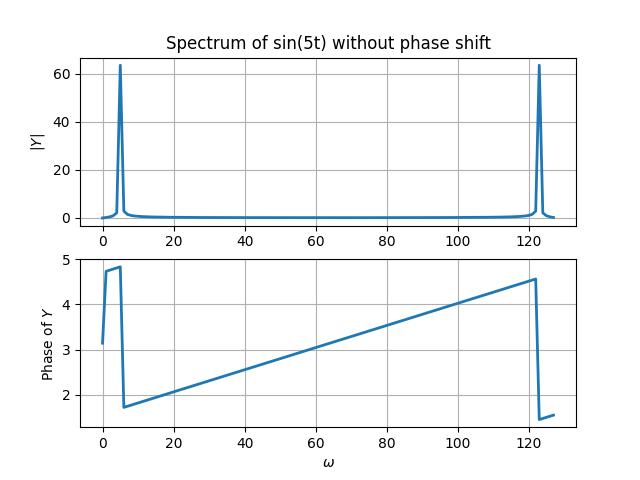
\includegraphics[scale=0.6]{Figure_1.png}
\caption{Spectrum of sin(5t) without Phase wrapping}
\label{fig:universe}
\end{figure}

\begin{figure}[h!]
\centering
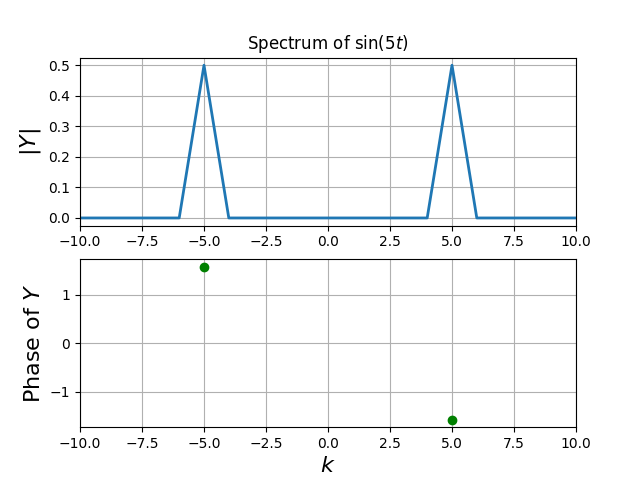
\includegraphics[scale=0.6]{Figure_2.png}
\caption{Spectrum of sin(5t) after phase wrapping}
\label{fig:universe}
\end{figure}


\clearpage
\subsection{Spectrum of Amplitude Modulated Wave}

\begin{equation}
f(t) = (1+0.1\cos(t))\cos(10t)    
\end{equation}

We note that 2 of the peaks have merged, we need to increase the number of samples we take. Calling the same function with a larger range and a higher number of samples we get 3 peaks.

\begin{figure}[h!]
\centering
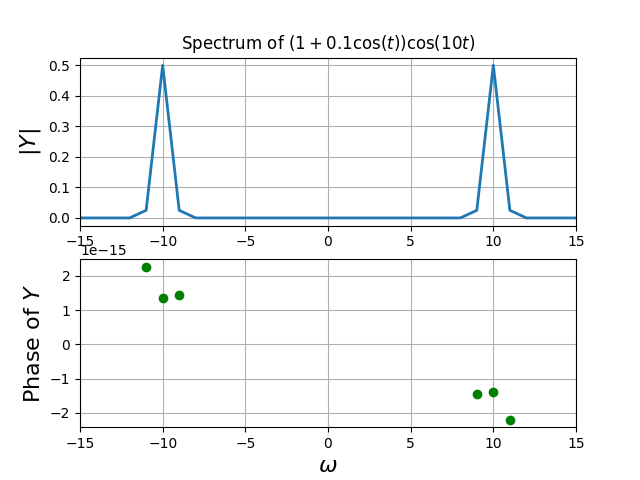
\includegraphics[scale=0.55]{Figure_3.png}
\caption{Spectrum of $(1+0.1\cos(t))\cos(10t)$ with low number of samples}
\label{fig:universe}
\end{figure}

\begin{figure}[h!]
\centering
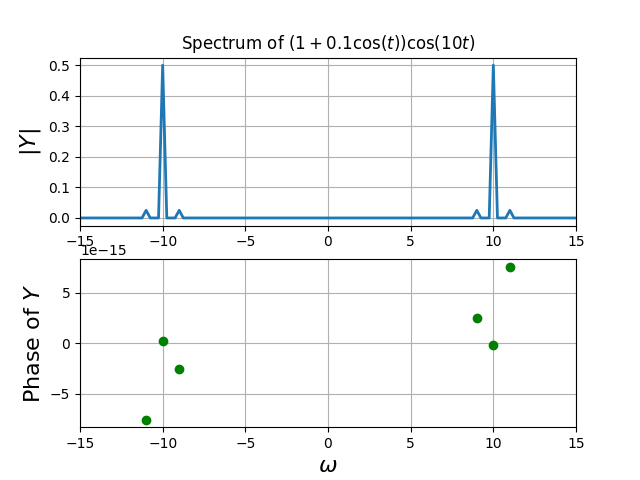
\includegraphics[scale=0.55]{Figure_4.png}
\caption{Spectrum of $(1+0.1\cos(t))\cos(10t)$ with a higher number of samples}
\label{fig:universe}
\end{figure}
\clearpage
\subsection{Spectrum of $sin^3(t)$}
This signal can be expressed as a sum of sine waves using this identity:\newline
$\sin^3(t) = \frac{3}{4}\sin(t) - \frac{1}{4}\sin(3t)$\newline
We expect 2 peaks at frequencies 1 and 3, and phases similar to that expected from a sum of sinusoids.
\begin{figure}[h!]
\centering
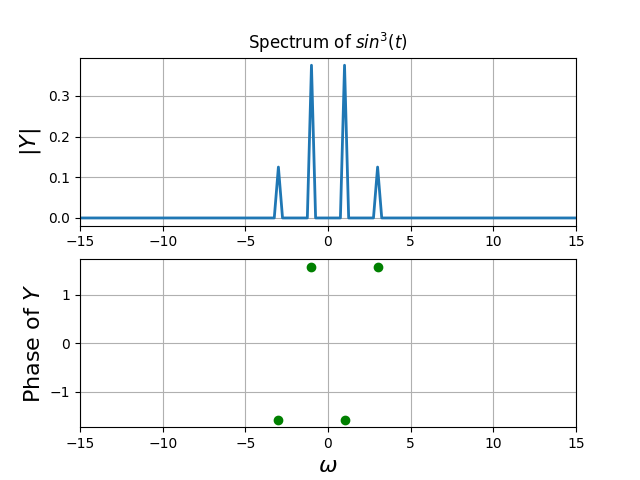
\includegraphics[scale=0.5]{Figure_5.png}
\caption{Spectrum of $sin^3(t)$}
\label{fig:universe}
\end{figure}

\subsection{Spectrum of $cos^3(t)$}
We expect 2 peaks at frequencies 1 and 3, and phase=0 at the peaks.
\begin{figure}[h!]
\centering
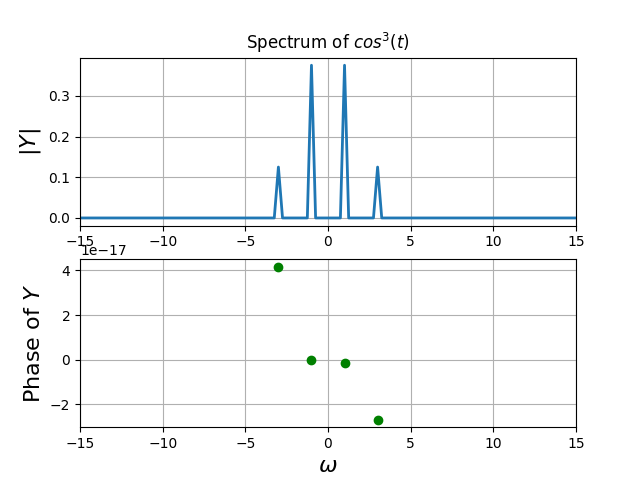
\includegraphics[scale=0.5]{Figure_6.png}
\caption{Spectrum of $cos^3(t)$}
\label{fig:universe}
\end{figure}
\clearpage
\subsection{Spectrum of Frequency Modulated Wave}
The number of peaks has clearly increased. The energy in the side bands is comparable to that of the main signal.
\begin{figure}[h!]
\centering
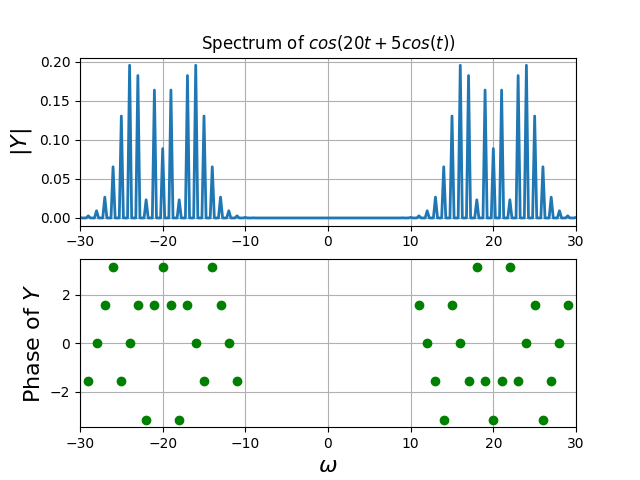
\includegraphics[scale=0.6]{Figure_7.png}
\caption{Spectrum of $cos(20t +5 \cos(t))$}
\label{fig:universe}
\end{figure}



\subsection{Continuous time Fourier Transform of a Gaussian}

The expression for the Gaussian is :
\begin{equation}
    x(t) = e^{\frac{-t^2}{2}}    
\end{equation}
The CTFT is given by:
\begin{equation}
X(j \omega) = \frac{1}{\sqrt{2 \pi}}e^{\frac{-\omega^2}{2}}    
\end{equation}



\begin{figure}[h!]
\centering
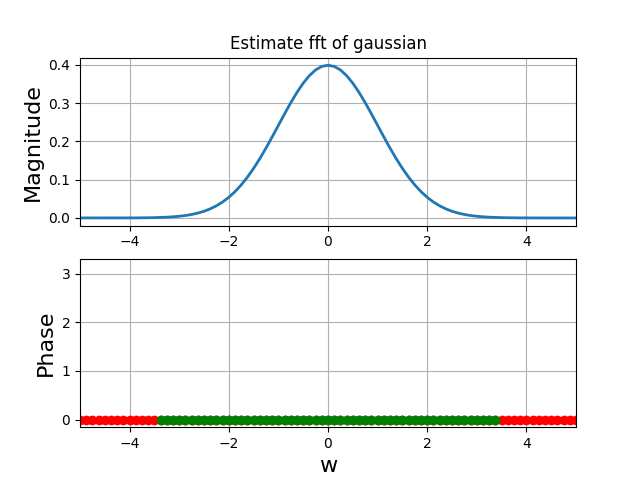
\includegraphics[scale=0.6]{Figure_8.png}
\caption{Estimated CTFT of Gaussian}
\label{fig:universe}
\end{figure}

\begin{figure}[h!]
\centering
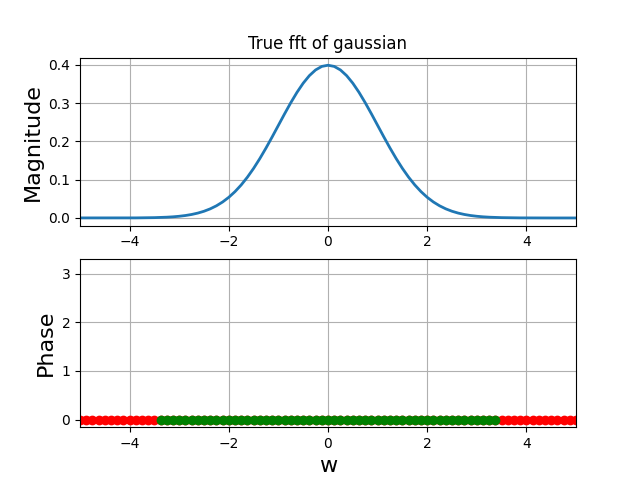
\includegraphics[scale=0.6]{Figure_9.png}
\caption{Expected CTFT of Gaussian}
\label{fig:universe}
\end{figure}
For $N=512, w_{lim}=32 rad/s$ \\
The summation of the absolute values of the error = 1.472553842671434e-14\newline


\clearpage

\section{Conclusion}


\begin{itemize}
\item The numpy.fft library on a random signal gives satisfactorily low error in the reconstructed signal.
	
\item There are multiple issues that need to be fixed in spectrum of sin(5t):

	• The peaks are not where we expect them to be. This can be corrected
	using fft shift.\\
	• The spikes have a height of 64, not 0.5. This should be rectified by
	dividing by the sample rate.\\
	• The frequency axis is not in place. This is due to the duplicacy of 0
	and 2$\pi$.\\
	• The actual phase at the spikes is near but not exactly correct.

\item In AM modulated signal, in order to see even the side peaks, the frequency resolution has to be improved. We can do so by keeping the number of samples constant and increasing the range in the time domain.

\item In the frequency spectrum of sinusoids, there will be 4 impulses, with on pair
at thrice the frequency than the other. Taking the same precautionary
measures as done previously, we obtain the following approximate spectrum.

\item Then we tried to iteratively estitmate the CTFT for a Gaussian signal. In each case, we utilise sampling of the DTFT to explain the spectrum or have used the discretisation of the continuous array the signal is derived from.There is a need for using ifftshift and fftshift to fix distorted phase responses.

\end{itemize}


\end{document}
